\section{Ejercicio 1}
\noindent
En la presente sección se tratará el diseño, construcción y medición de un circuito que controla un sistema de dos bombas de agua en base a las señales enviadas por dos sensores, uno ubicado en la parte superior de un tanque de agua, y el otro ubicado en la parte inferior del mismo. Así las señales de los sensores dominan los ciclos de trabajos de las bombas, de tal forma que las bombas alternen sus ciclos de trabajo.\\
%
De esta manera se procedió a realizar una FSM que permita analizar la lógica detrás del circuito a realizar, así, la FSM que controla al sistema se puede ver en la figura \ref{ej1_fsm}, el mismo está realizado con una maquina de Moore.
%
\begin{figure}[H]
    \centering
    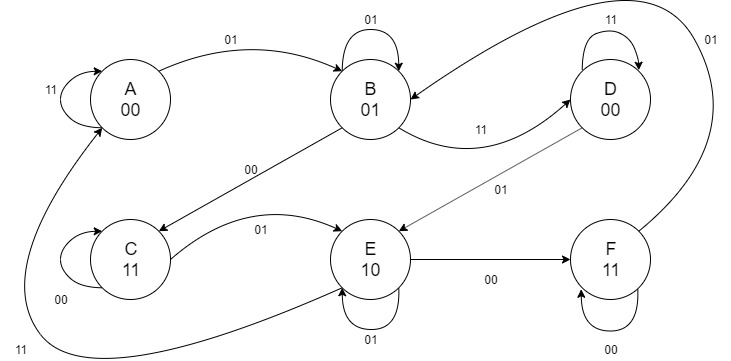
\includegraphics[width=0.7\textwidth]{figs/Ej1/diagrama_grande.jpg} % first figure itself
    \caption{Digrama de estados de la FSM}
    \label{ej1_fsm}
\end{figure}
%
\noindent
De esta manera podemos ver como el diagrama de estados que controla ambas bombas presenta 6 estados, por lo tanto necesitará de al menos 3 flip flop ademas de los componentes lógicos que permitan diseñar la lógica necesaria del sistema. Se consideró por lo tanto que esta solución era ineficiente y por lo tanto se procedió a implementar una FSM de menor tamaño que controle una parte del sistema en cuestión en lugar de todo el sistema como en el caso anterior.\\
Así lo que se realizó fue una FSM que segun las entradas de las señales de los sensores de agua del tanque, entrega 2 salidas posibles, una indica que ambos motores se encuentran encendidos y la otra indica que sólo un motor debe ser encendido. De esta manera luego con ayuda de lógica externa mediante un flip flop T se implementa la lógica correspondiente a la alternancia de los ciclos de trabajo de las bombas.\\
%
Por lo tanto el diagrama de estados correspondiente a este nuevo enfoque del problema se puede ver en la figura \ref{ej1_fsm2}
%
\begin{figure}[H]
    \centering
    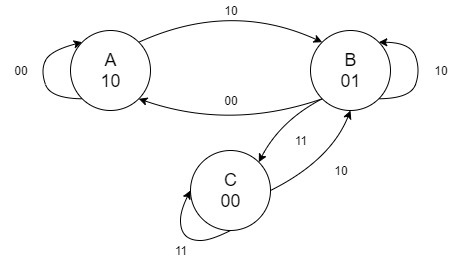
\includegraphics[width=0.7\textwidth]{figs/Ej1/diagrama_chico.jpg} % first figure itself
    \caption{Digrama de estados de la FSM utilizada.}
    \label{ej1_fsm2}
\end{figure}
%
\noindent
Así, la tabla de estados del diagrama se puede ver en la tabla \ref{ej1_tabla}.
%
\begin{table}[H]
\centering
\caption{Tabla de estados.}
\label{ej1_tabla}
\begin{tabular}{|c|c|c|c|c|c|c|}
\hline
\multicolumn{2}{|c|}{Estado Actual}             & \multicolumn{4}{c|}{Estado Siguiente} & Salida                           \\ \hline
\multirow{2}{*}{Nombre} & \multirow{2}{*}{y1y2} & I=0,S=0 & I=0,S=1 & I=1,S=0 & I=1,S=1 & \multirow{2}{*}{Ambas, Solo Una} \\ \cline{3-6}
                        &                       & Y1Y2    & Y1Y2    & Y1Y2    & Y1Y2    &                                  \\ \hline
A                       & 00                    & 00      & XX      & 10      & XX      & 10                               \\ \hline
B                       & 10                    & 00      & XX      & 10      & 11      & 01                               \\ \hline
C                       & 11                    & XX      & XX      & 10      & 11      & 00                               \\ \hline
X                       & 01                    & XX      & XX      & XX      & XX      & XX                               \\ \hline
\end{tabular}
\end{table}
%
\noindent
Así los mapas de karnaugh resultantes se pueden ver a continuación, donde a y b corresponden a y1 e y2 mientras que c y d corresponden a I y S es decir los sensores inferior y superior respectivamente.\\
%
Y1:
\begin{center}
\begin{Karnaugh}
    \minterms{8,10,11,14,15}
    \indeterminats{1,3,4,5,6,7,9,12,13}
    \maxterms{0,2}
    \implicant{12}{10}{red}
\end{Karnaugh}
\end{center}
%
Y2:
\begin{center}
\begin{Karnaugh}
    \minterms{14,15}
    \indeterminats{1,3,4,5,6,7,9,12,13}
    \maxterms{0,2,8,10,11}
    \implicant{4}{14}{green}
\end{Karnaugh}
\end{center}
%
Ambas:
%
\begin{center}
\begin{Karnaughquatre}
    \minterms{0}
    \indeterminats{2}
    \maxterms{1,3}
    \implicant{0}{2}{yellow}
\end{Karnaughquatre}
\end{center}
%
Solo una:
%
\begin{center}
\begin{Karnaughquatre}
    \minterms{1}
    \indeterminats{2}
    \maxterms{0,3}
    \implicantsol{1}{blue}
\end{Karnaughquatre}
\end{center}
%
\noindent
De esta manera las expresiones lógicas resultantes se pueden ver en las ecuaciones \ref{ej1_eq1}.
%
\begin{equation}
\begin{split}
    Y1&=I\\
    Y2&=S\\
    Ambos&=\overline{y1}\\
    Solo\hspace{1mm}uno&=y1\overline{y2}
\label{ej1_eq1}
\end{split}
\end{equation}
\noindent
Por lo que el diagrama del circuito a realizar se puede ver en la figura \ref{ej1_circuito1.}
%
\begin{figure}[H]
    \centering
    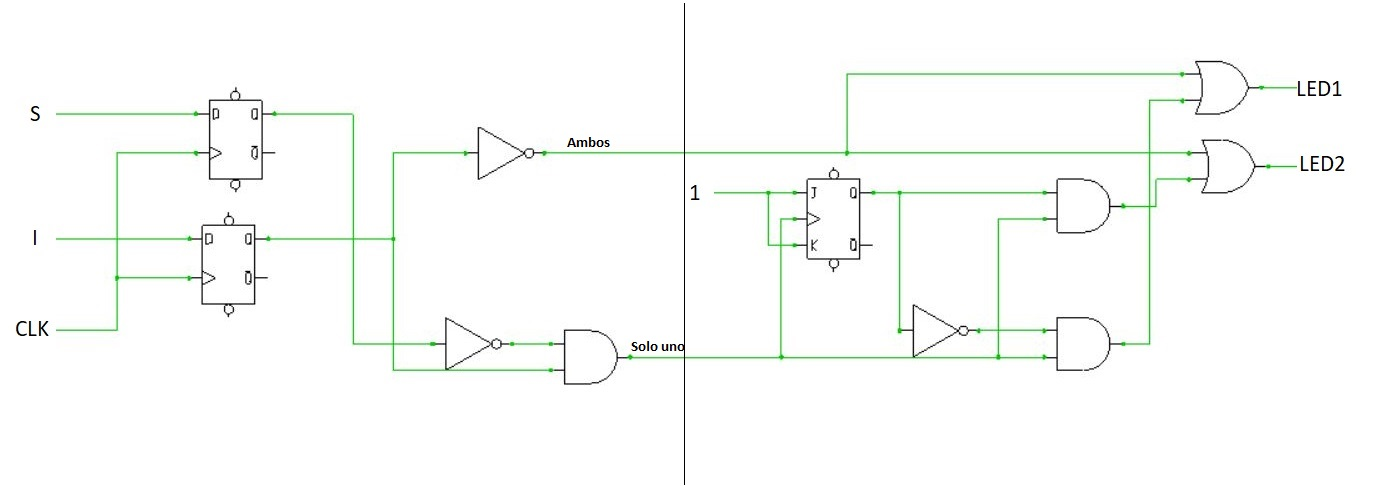
\includegraphics[width=0.9\textwidth]{figs/Ej1/circuitofacilfacil.JPG} % first figure itself
    \caption{Circuito realizado mediante las simplificaciones del mapa de Karnaugh}
    \label{ej1_circuito1.}
\end{figure}
%
\noindent
En el circuito mostrado toda la lógica siguiente a la linea vertical negra corresponde a la utilizada para realizar la alternancia de los ciclos de trabajo de las bombas (LEDS), para ello se utilizó un flip flop JK con la finalidad de construir el Flip flop T necesario del sistema.\\
Se puede notar además en el dibujo de la figura anterior que se puede evitar el uso de ambos flip flop debido a que el sistema no necesita ser sincrónico para funcionar debido a que contempla la entrada asincrónica de las señales de los sensores de los tanques de agua y las salidas asincrónicas de los encendidos de los motores. De todas formas si el sistema requiriese una salida sincrónica porque se conecta con otros sistemas que trabajan de esta forma entonces los flip flops sí serían necesarios. \\
A continuación se muestra el circuito sin el uso de flip flops D.
%
\begin{figure}[H]
    \centering
    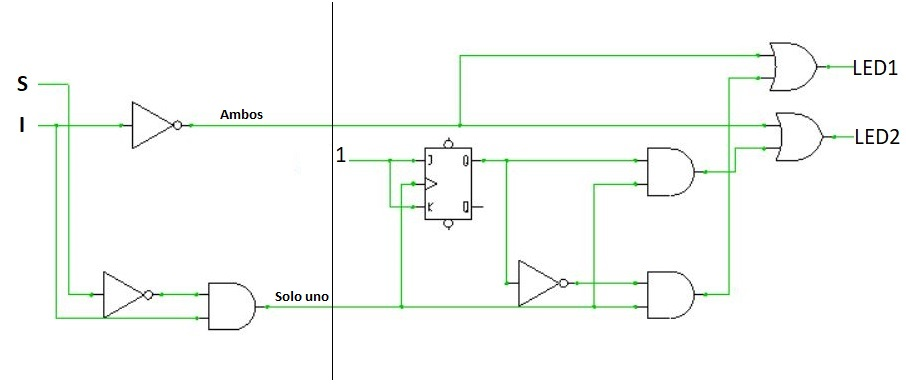
\includegraphics[width=0.9\textwidth]{figs/Ej1/circuito_facil.JPG} % first figure itself
    \caption{Circuito realizado mediante las simplificaciones del mapa de Karnaugh sin los flip flops.}
    \label{ej1_circuito2.}
\end{figure}
%
De esta forma y con la finalidad de ahorrar integrados se realizaron simplificaciones de componentes para lograr utilizar sólo el flip flop jk y compuertan nand, de esta manera el resultado se puede ver en la figura \ref{ej1_circuito3.}.
%
\begin{figure}[H]
    \centering
    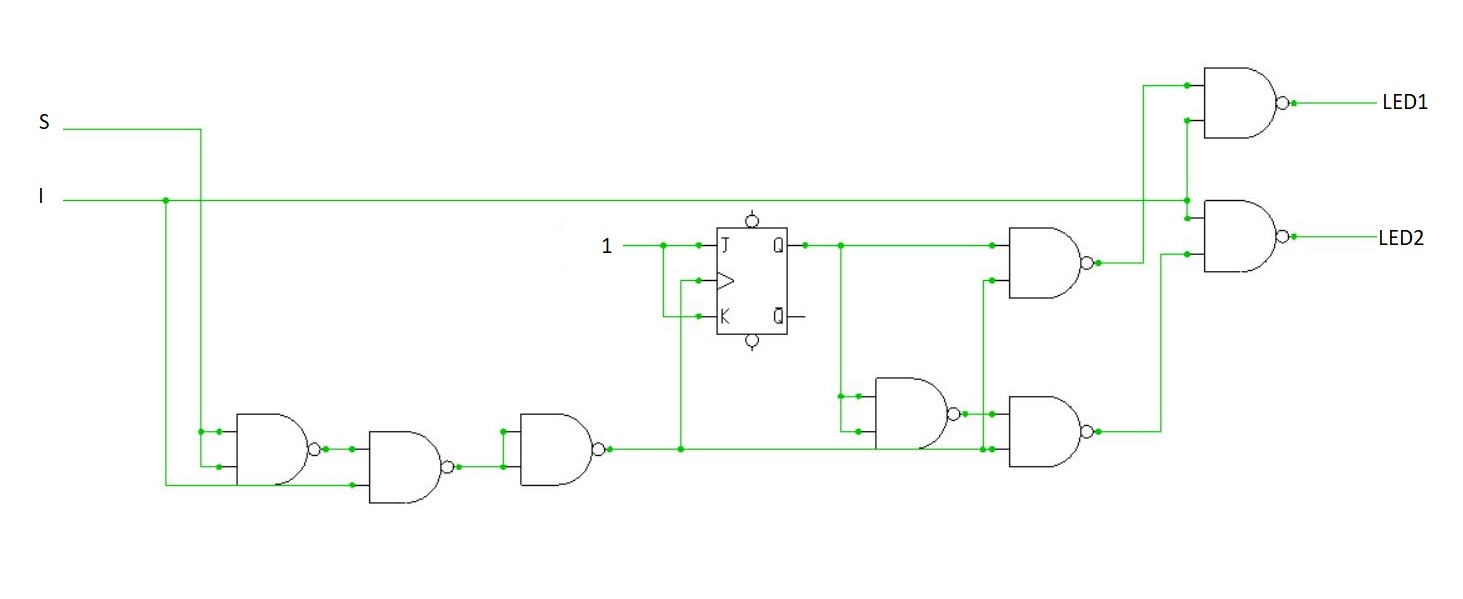
\includegraphics[width=0.9\textwidth]{figs/Ej1/circuito.JPG} % first figure itself
    \caption{Circuito realizado mediante las simplificaciones del mapa de Karnaugh sin los flip flops.}
    \label{ej1_circuito3.}
\end{figure}
%
\noindent
Así, se implementó el circuito en una placa PCB mediante 2 integrados para las compuertas nand, un integrado para el flip flop jk necesario, para las entradas se utilizaron 2 jummpers conectados mediante una resistencia pull down al sistema y a la salida se dispuso de un LED conectado a tierra y al sistema mediante una resistencia que controla la corriente que circula por dicho LED.\\
Los resultados encotrados fueron los esperados, el sistema se comporta fielmente con lo esperado para el mismo.\\
Se anexa en la carpeta de este trabajo un video mostrando el funcionamiento de la placa PCB en cuestión.